\chapter{Results}
\startcontents[chapters]

\section{Descriptive statistics}
The first hypothesis this study aims to test is: there is a monotonous shift from one value of gender to another when going from attributive, through predicate to relative pronoun agreement. Additionally, the hypothesis proposed with the definition of generalized semantic agreement will be tested, which is that split hybrids (here the depreciative forms) are less likely to have generalized semantic agreement than lexical hybrids (here the socially gendered nouns and profession nouns). Before those hypotheses are addressed, let us look at the dataset extracted from the corpus. 

A total of 199 927 observations of agreement have been collected, although a vast majority of them was agreement with profession nouns, for which it was impossible to clearly determine whether it was hybrid agreement or not, as this would require manually finding the referent of the noun from the context. Because of that, only profession nouns with feminine agreement were used in the analysis. The summary of the types of agreements and controllers found in the dataset is in Tables \ref{tab:summary-agreements} and \ref{tab:summary-controllers} respectively. 

\begin{table}
  \centering
  \begin{tblr}
    {
      hlines,vlines,
      row{1} = {gray9},
    }
  Type of agreement & N & Percentage \\
  attributive & 1873 & 52.627\% \\
  predicative & 1478 & 41.529\% \\
  relative pronoun & 208 & 5.844\% \\
  \end{tblr}
  \caption{Numbers and percentages of different types of agreement in the dataset.}
  \label{tab:summary-agreements}
\end{table}

\begin{table}
  \centering
  \begin{tblr}
    {
      hlines,vlines,
      row{1} = {gray9},
    }
  Type of controller & N & Percentage \\
  depreciative & 1040 & 29.222\% \\
  gendered & 807 & 22.675\% \\
  profession & 1712 & 48.103\% \\
  \end{tblr}
  \caption{Numbers and percentages of different types of controllers in the dataset.}
  \label{tab:summary-controllers}
\end{table}

First, we will look at proportions of semantic agreement with attributive, predicate and relative pronoun targets, which are visualized by Figure \ref{fig:proportions}. Semantic agreement was favored in predicate agreement with both depreciatives and socially gendered nouns. This is contrary to the hypothesis about monotonous shift from one value to another along the agreement hierarchy, but this will be further addressed in the next section.

\begin{figure}
  \centering
  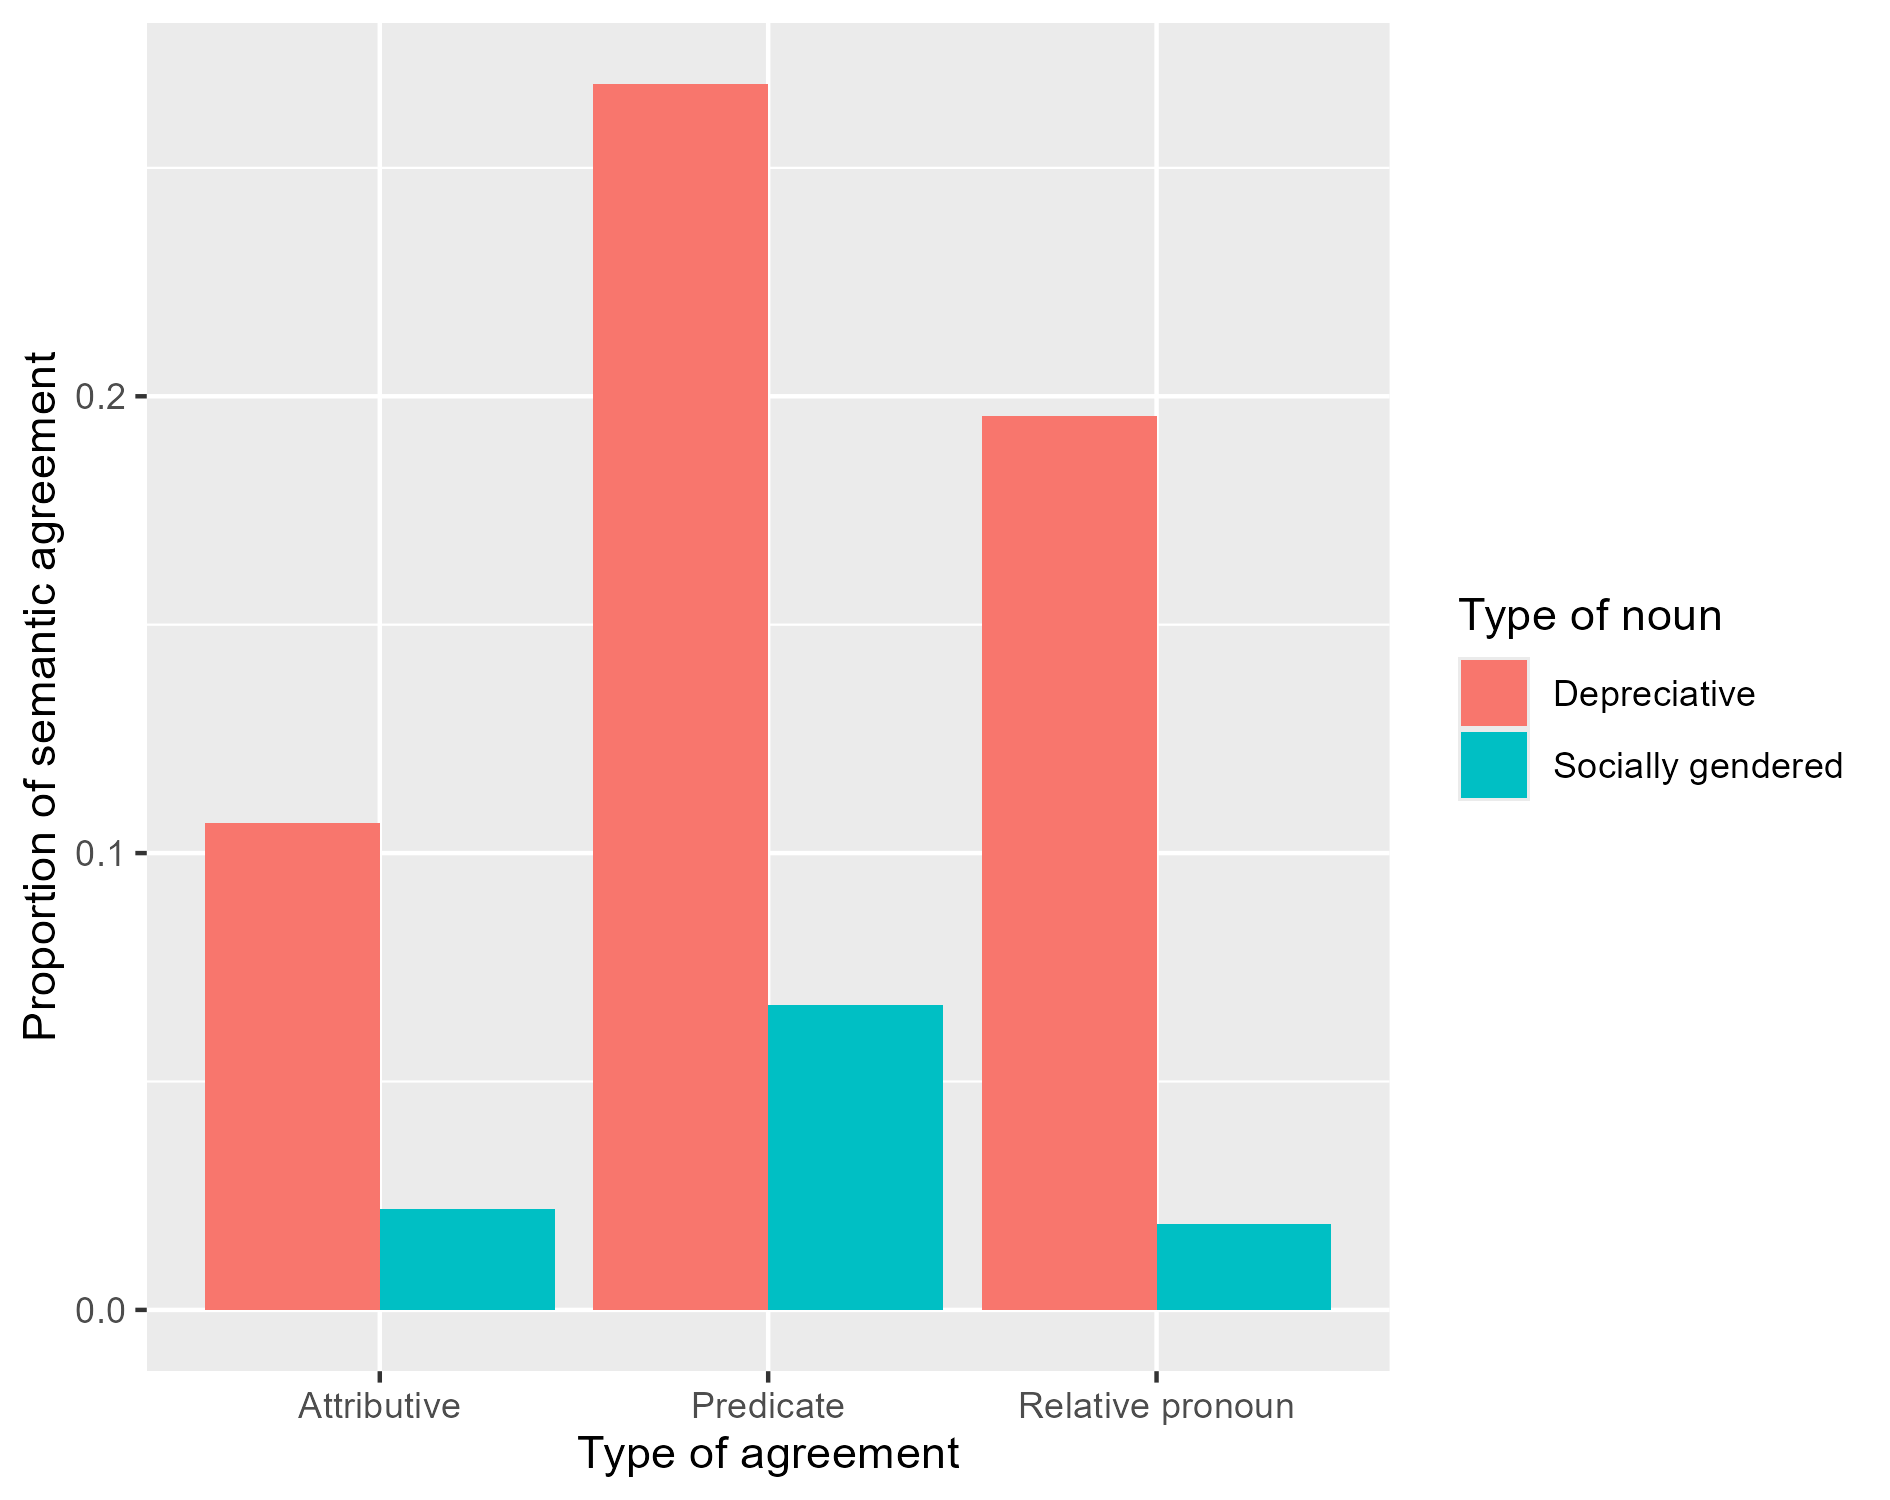
\includegraphics{images/props.png}
  \caption{Proportions of semantic agreement for each type of agreement for socially gendered and depreciative nouns.}
  \label{fig:proportions}
\end{figure}

For profession nouns only feminine agreement is considered, which means all of the examples have semantic agreement, so these occurrences cannot be reported in a similar figure. It can be reported, however, how many of the semantic agreement occurrences with profession nouns were attributive, predicate and relative pronoun agreement. This can be found in Table \ref{tab:prof-summary}. We can see a similar number of attributive and predicate, but very few relative pronoun agreements.

\begin{table}
  \centering
  \begin{tblr}
    {hlines, vlines,
    row{1} = {gray9}}
    Type of agreement & N & Percentage \\
    Attributive & 845 & 49.357\% \\
    Predicate & 758 & 44.276\% \\
    Relative pronoun & 109 & 6.367\% \\
  \end{tblr}
  \caption{Number of different types of agreement found with profession nouns along with their percentages among the semantic agreements with profession nouns}
  \label{tab:prof-summary}
\end{table}

Figure \ref{fig:distance} shows the average distance between the target and the controller of agreement measured as the number of intervening words. It was the largest in predicate agreement for both depreciatives and socially gendered nouns. The exact average distances can be found in Table \ref{tab:distance}. It was most common for attributive agreements to have the target before the controller (73.5\%), with predicate agreements it happened in 30.2\% of cases. There were 11 occurrences of target before controller in relative pronoun agreement, but those have been a result of parsing errors since it it not possible to put a relative pronoun before the noun to which it refers. 

\begin{figure}
  \centering
  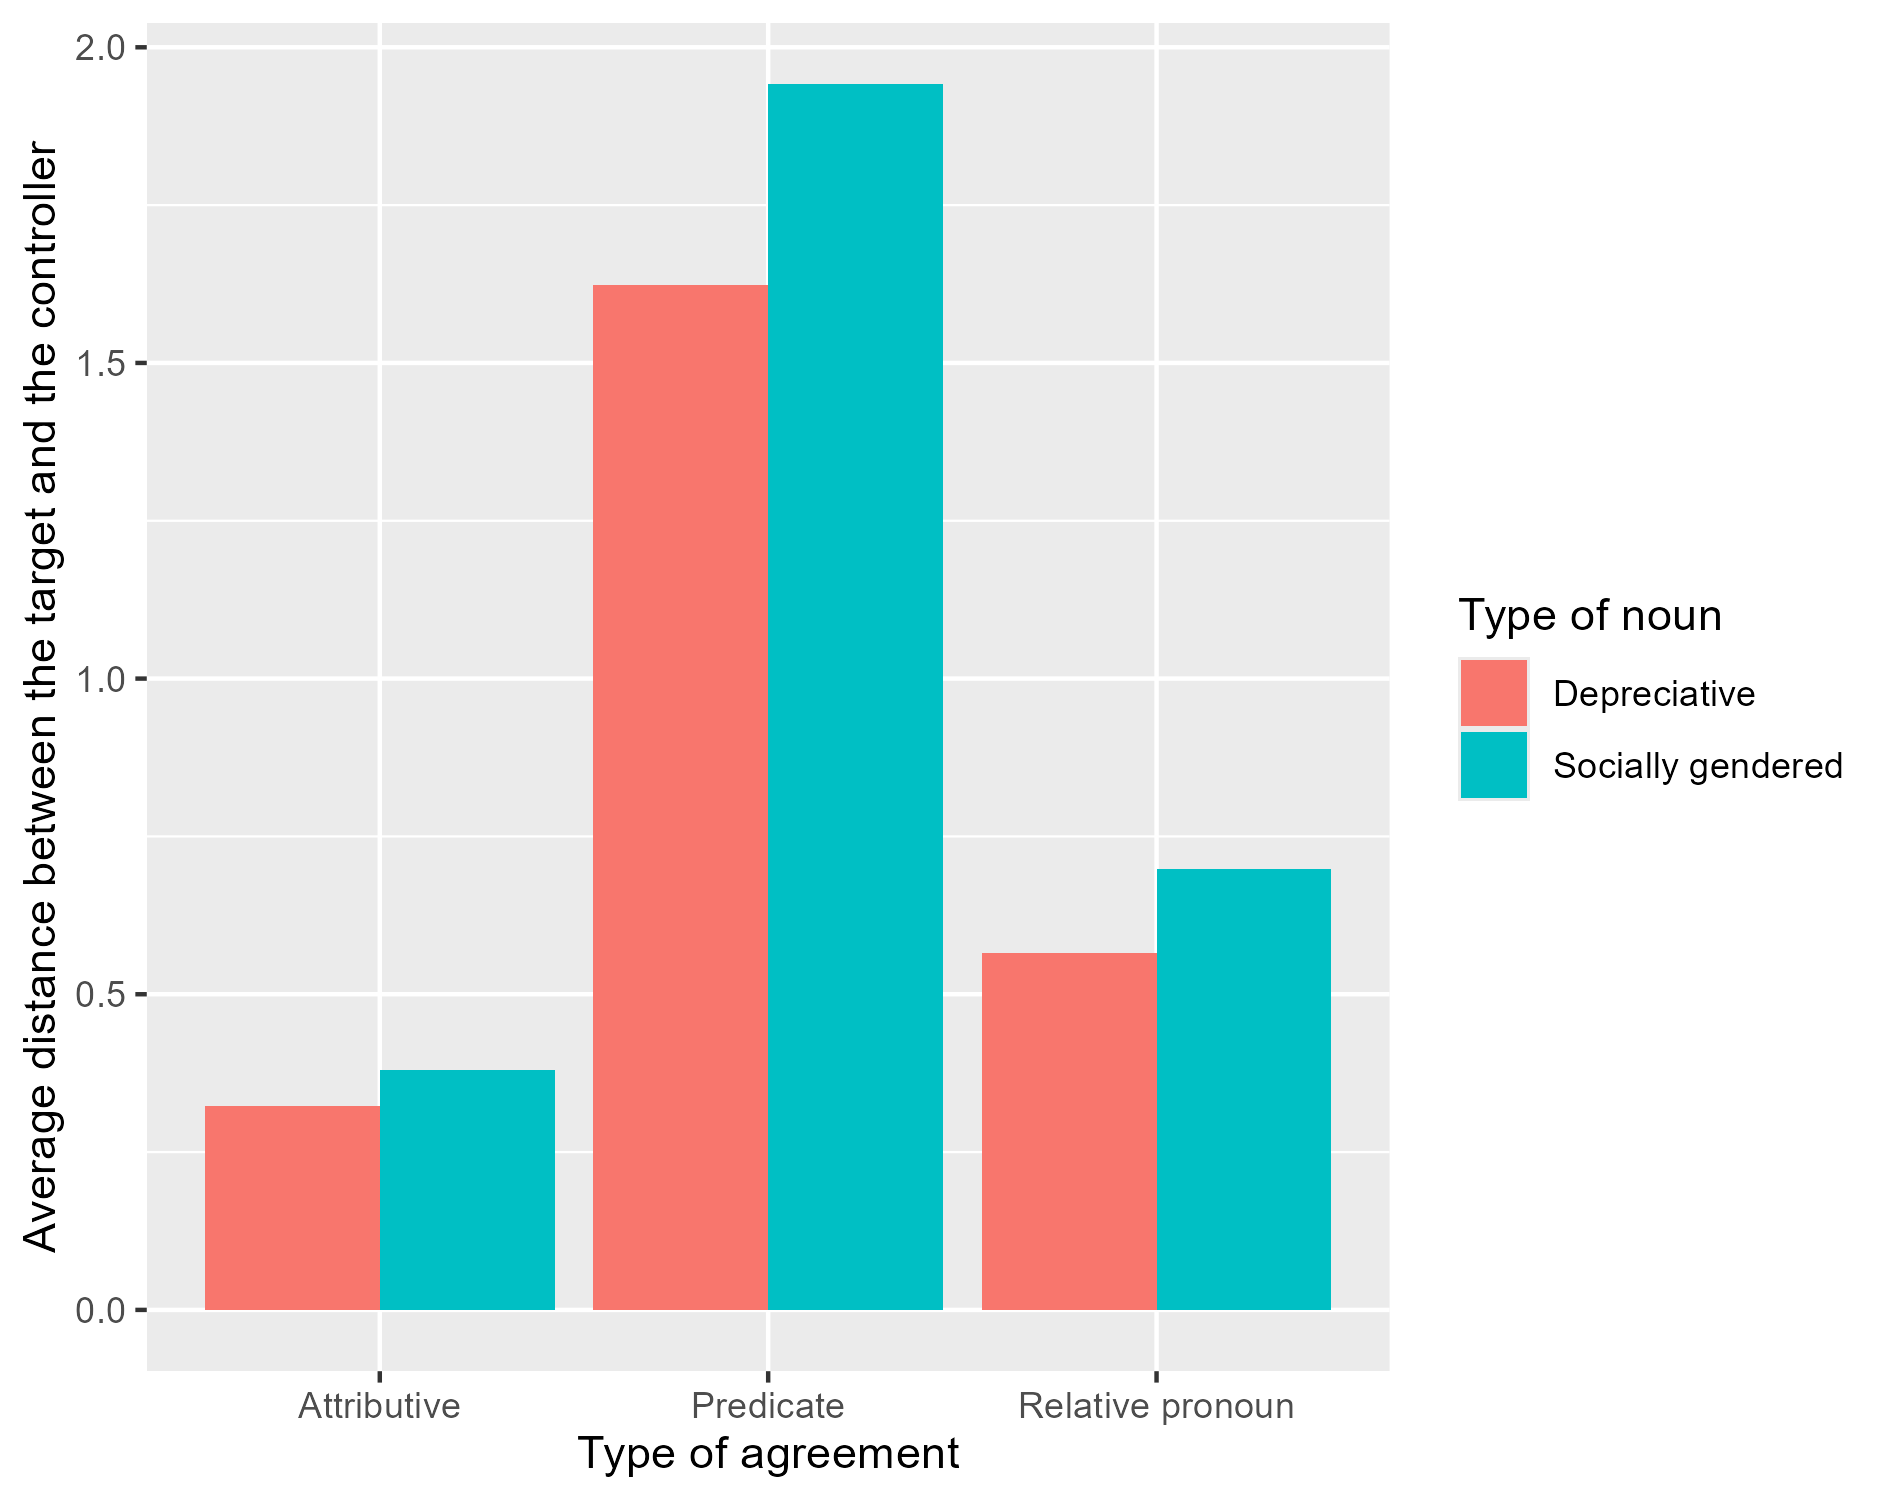
\includegraphics{images/dist.png}
  \caption{Average distance between the target and the controller of agreement for each type of agreement and for each type of noun.}
  \label{fig:distance}
\end{figure}

\begin{table}
  \centering
  \begin{tblr}
    {
      hlines,vlines,
      row{1} = gray9,
      cell{2}{1} = {r=2}{l},
      cell{4}{1} = {r=2}{l},
      cell{6}{1} = {r=2}{l},
    }
    Type of agreement & Type of noun & Average distance \\
    attributive & depreciative & 0.3223350 \\
    attributive & gendered & 0.3801262 \\
    predicative & depreciative & 1.6233333 \\
    predicative & gendered & 1.9416667 \\
    relpron & depreciative & 0.5652174 \\
    relpron & gendered & 0.6981132 \\
  \end{tblr}
  \caption{Average distance between the target and the controller in all types of nouns and agreements as shown in Figure \ref{fig:distance}.}
  \label{tab:distance}
\end{table}

As for the hypothesis regarding the hierarchy of agreement sources, 20.4\% of agreements with depreciatives had semantic agreement, while it was only 2.85\% for socially gendered nouns. This is further looked into in the following section.

It should be noted there were 15 profession nouns that did not have semantic agreement at all. Those nouns, along with their translations to English, can be found in Table \ref{tab:prof-zero}.

\begin{table}
  \centering
  \begin{tblr}
    {
      hlines, vlines,
      row{1} = {gray9},
      column{2} = {.4\hsize},
    }
    Lexeme in Polish & Translation to English & No. of occurrences \\
    demiurg & demiurge & 119 \\
    dramaturg & playwright & 397 \\
    elekt & person elected in a specified post, but has not yet entered office & 14 \\
    foniatra & phoniatrician & 2 \\
    ftyzjatra & pulmonologist & 1 \\
    geometra & geometer & 39 \\
    geriatra & geriatrician & 3 \\
    jaskiniowiec & caveman & 35 \\
    metalurg & metallurgist & 8 \\
    murarz & bricklayer & 241 \\
    muzykolog & musicologist & 80 \\
    nieuk & dunce & 37 \\
    nurek & diver & 109 \\
    pajac & clown & 10 \\
    szklarz & glazier & 50 \\
  \end{tblr}
  \caption{Table of profession nouns (and their translations and numbers of occurrences in the corpus), for which there was no semantic agreement found in the dataset.}
  \label{tab:prof-zero}
\end{table}
  
\section{Statistical models}

The models discussed in this section are not based on the profession nouns, since a vast amount of data in this category contained occurrences of the nouns that could not have hybrid agreement and could not have been filtered out automatically. The following analysis is based only on the agreements with depreciative forms and socially gendered nouns.

The analysis was conducted using the \texttt{glm} function from the \texttt{lme4} R package. Models computed using this function were all binomial generalized linear models, because the dependent variable was binary: whether semantic agreement was chosen or not. There were 4 variables tested as predictors for semantic agreement in separate generalized linear models. Those variables were: type of agreement (attrbutive, predicate, relative pronoun), distance between the target and the controller, target preceding the controller and type of controller noun (socially gendered or depreciative). No random factors were included. The formulae used for the models as well as the full output can be found in the Appendix. 

The model predicting based on the type of agreement showed that predicates favor semantic agreement more than attributives (estimate = -1.6722, p < 2e-16), but relative pronouns favor semantic agreement less than predicates (estimate = 1.0042, p = 0.0036), which does not show a monotonous shift from one value of gender to the other, as was expected. The model based on the distance gave expected results on the other hand, the larger the distance between the target and the controller, the more likely it is the semantic agreement will be chosen (estimate = 0.14115, p = 2.32e-06). According to the model predicting based on the ordering of the target and the controller, target being before the controller lowers the likelyhood of semantic agreement (estimate = -1.53658, p < 2e-16). Finally, the socially gendered nouns are less likely to have semantic agreement than the depreciatives (estimate = -2.1664, p < 2e-16).

Additionally, a multivariable model using the same 4 variables as predictors was computed. Estimates and p-values from this model are presented in Table \ref{tab:multivar-model}, the formula and full output of the model can be found in the Appendix. According to this model, when considering the interaction between all the predictors, only some of them are statistically significant. Predicate agreement favors semantic agreement, while socially gendered nouns do not. Target appearing before the controller also discourages from using semantic agreement.

\begin{table}[H]
  \centering
  \begin{tblr}
    {
      vlines,hlines,
      column{2,3} = {r},
      row{1} = {c, gray9},
    }
    Predictor & Estimate & P-value \\
    Predicate agreement & 0.45490 & \textbf{0.0345} \\
    Relative pronoun agreement & -0.21101 & 0.5959 \\
    Distance & 0.03983 & 0.2191 \\
    Ordering & -0.99116 & \textbf{1.59e-06} \\
    Type of noun: gendered & -1.73335 & \textbf{3.77e-13} \\
  \end{tblr}
  \caption{Estimates and p-values assigned to all predictors in the multivariable model. Predictors, that are statistically significant at the 0.05 level are bolded.}
  \label{tab:multivar-model}
\end{table}
